\documentclass[12pt]{article}
\usepackage{geometry}
%\geometry{left = 3cm, right = 2.5cm, top = 2.5cm, bottom = 2.5cm}
\usepackage{graphicx}
\usepackage{cite}
\title{Improved genetic algorithm for finding shortest paths problem}
\author{Qi Yixi}
\date{\today}
\begin{document}
%\huge
\maketitle{}
\section{Introduction}
%\subparagraph{
	The optimal path problem is a very classical mathematical problem, which is the basis for many optimization problems such as resource allocation, path analysis and design. The shortest path algorithm can be divided into a single vertex shortest path algorithm, and a shortest path algorithm between each pair of vertices. A typical solution to converntional route planning problems is the Dijkstra algorithm, which has used in road networks and in dynamic environments to find a route minimizing the travel time from an origin to a destination. However in the practical application, the size of the shortest path problem is expanding, the constraint condition of the shortest path problem is increasing. In the traditional algorithm, it is difficult to effectively find a perfect solution to quickly find the optimal solution or suboptimal solution, and then some study use the genetic algorithm to find the shortest path.
\subsection{Genetic algorithm}
Genetic algorithm is a computational model simulating the natural selection and genetic mechanism of Darwinian biological evolution, and it is a method to search the optimal solution by simulating the natural evolution. Genetic algorithm starts from a population which represents the potential solution set of the problem, and a population is composed of a certain number of individuals encoded by gene. The steps of the Genetic algorithm are firstly generation some population. After the generation of the first generation of population, according to the survival of the fittest and the survival of the fittest, generation evolves generation by generation to produce better and better approximate solutions. In each generation, individuals are selected according to the fitness of individuals in the problem domain, and with the help of nature. Genetic operators in genetics carry out cross and mutation to produce populations representing new solution sets. This process will result in the population of the posterity, like the natural evolution, more adaptable to the environment than that of the previous generation. The optimal individuals in the last generation can be decoded as the approximate optimal solution of the problem. Genetic algorithm generates many solutions to a single problem each one with different performance some are better than other in performance. So it have been successfully applied to many search, optimization, and machine learning problems. The evolutionary process consists of maintaining a population of coded solutions which are manipulated by variation operators to find a satisfactory optimized solution. Such as find path, the writer used GA to help the robot path planning\cite{Alnasser2016}, and then they find the GA is more efficiency and effectiveness. 
Many studies using genetic algorithm to solve multi-objective route planning problems have been reported, which include a review of recent issue and applications to mobile robots, personal navigation, tourist sight sight-seeing itinerary and personal navigation.    in the other hands, the JunWoo\cite{Kim2019} kim studies the candidate order based genetic algorithm to solve the maze-type shortest path problem, and then the author compared Fitness Switching Genetic Algorithm and Candidate Order based Genetic Algorithm. 
\subsection{Pruning algorithm}
In the optimization of search algorithm, pruning is to avoid some unnecessary traversal through some judgment. Generally speaking, it is to prune some "branches" in the search tree, so it is called pruning. The core problem of applying pruning optimization is to design pruning judgment method, that is, to determine which branches should be abandoned and which should be retained. The pruning algorithm often used in some machine learning algorithm\cite{Hu2019}, which achives the high-quality uncertainty estimation with a small value. In the other hand, the pruning stratages used in some tree problems and some search path problem.One of the questions that arises in the tree problem is the optimal size of the final tree. A tree that is too large risk overfitting the training data and poorly generalizing to new samples. A small tree might not capture important structural information about the sample space. In the genetic algorithm, this problem is more important, Although the algorithm has fitness function to judgement the final tree, however, to prevent miss the optimal path, the genetic algorithm need to produce more and more offspring. Pruning not only can reduce the save offspring, but also can keep the find path accuracy. 
At present, the pruning algorithm is widely used in machine learnning and the decision tree or greedy algorithm. In the past years, most study use the pruning algorith to save the tree problem. For example, Yasuo\cite{Yamane2019} make a new
fast unweighted all-pairs shortest path search algorithm, which combined the pruning algorithm and the breadth-first search, the result mention that the new algorithm more effectiveness than the traditional one. And then based on this study, they improved the algorithm\cite{Yamane2019a} and make it can fit the weight all-pair shortest path search problem. As mentation earlier, pruning algorithm is also often used for branching of decision trees. For reduce the feature cost\cite{Nan2016}, researcher use the pruning algorithm to prun the decision, at the results, they test the algorithm in the 0-1 integer problems, in the test, it is able to significantly reduce feature cost by pruning subtrees that introduce more loss in terms of feature cost than benefit in terms of prediction accuracy gain.  In the other hand, the pruning algorithm is also often used in the field of machine learning, researcher gave an pareto deep ensemble pruning model\cite{Hu2019} , it can save the uncertainty prediction problems and effectively get the results.  
In some other ways, some research use this algorithm\cite{10.1007/978-3-642-28493-9_10}, which writer used the tree-delection pruning in the real-world road networks. However, more research is biased towards the pruning algorithm used by machine learning rather than simply using the pruning algorithm to optimize the genetic algorithm. For example, the Weight Pruning Genetic Algorithm\cite{Janjic2019}, thie paper use the pruning algorithm to pruning specific mutators to optimizing neural networks. In this paper, we will use the pruning algorithm to improved the genetic algorithm.

\section{Research purposes}
%\subparagraph{
Traditional genetic algorithm always used in the machine learning, in the past years, people find it can use in the find path problem, With the graph point grow, the genetic algorithm has the less time cost than the dijkustra algorithm. However, with the graph increase, there is more computing consumption\cite{10.1007/978-3-319-74521-3_20}. For reduce the computing consumption, this paper will use the pruning algorithm. In order to get the best answer, the traditional genetic algorithm needs to generate a large number of offspring, it may cost more save space and the more computation, using pruning algorithm may solve this problem.

\section{Related research}	
%\subsection{Genetic algorithm}
%\subparagraph{
Techniques  like Dijkstra, Floy-warshall and Bellman ford are the most commonly used algorithms for evaluating shortest paths. especially the Dijkstra, not only in the static environment, but also in the dynamic environment[], the Dijkstra was the most popular algorithms in the past years. Whith the time goes by, the amount of data that needs to be processed is also increaing, compared to the Dijkstra algorithm, the genetic algorithm have the better resulty to solve the big data shortest path problem[]. So some studies have begun to focus on solving the shortest path  problem with genetic algorithm. In the recently, one research using GAs to solve the supermarket manger traveling problem\cite{Al-hayali2018}.This is one of the shortest path problem,the writer makes a GAs models and then use an example to show the GAs is an efficient method to provide optimizations of these problems.
in the other hand, study impoved the genetic algorithm and use  improved GAs to solve the multi-objective route planning problems in dynamic problems\cite{Kanoh2008}, and then he compared with traditional GAs and Dijkstra algorithm, the improved GAs cost a less time than DA. However, regardless of the purpose of their use of the genetic algorithm it is inevitable that one problem is that the data volume of the genetic algorithm is too large, because the genetic algorithm generates a large amount of offspring data. For solve this problem, some study use the different crossover strategy[], and the result present that cost less time than traditional genetic algorithm. In the other hand, some study try to change the 
%%%%%%% 
The shortest path problems always a Genetic algorithm starts from a population which represents the potential solution set of the problem, and a population is composed of a certain number of individuals encoded by gene. 

%\subsection{The pruning algorithm}
  




%\subsection{Dijkstra algorithm}

A type solution to conventional route planning problems is the Dijkstra algorithm(DA), which has been used in road networks and in dynamic environments to find a route minimizing the travel time from an origin to a destination. The main feature of Dijkstra algorithm is to extend from the starting point to the end. In the past ten years, more and more people use the algorithmt to make life better, they use the algorithm in the every aspect of life, such as cargo navigation, mine rescue shortest path. With the time go on, people try to use DA to solve some dynamic problem\cite{10.1007/978-3-319-60042-0_15}. However there also have some trouble in the DA, such as the most cost. To imporved the time cost, reseacher use Folyed-warshall algorithm and GA to find the best rout for the emergency patient\cite{Risald2017}. 



\section{Research plan}
%\subparagraph{
Implementation Genetic algorithm, which following step is in the figure1
1. Implementation the genetic algorithm as fllow steps:
\subsection{Coding and decoding}
%\subparagraph{
Coding the all of the graph point. Randomly generate sequences to form the original chromosome as the initial population, the length is the total number of points in the graph. Then use the depth traversal algorithm to get the decoding shortest path based on the node id.
\subsection{Set the fitness function}
%\subparagraph{
The fitness function is an important section in the genetic algorithm. From the table 1, the fitness function needs to calculate the individual fitness value, and then judgment the direction of evolution. Use fitness function can choose the best individual and then choses the generate direction. From the recently study\cite{Gunturu2017}, the reasercher use the fitness function to find game equilibria, the result proposed  fitness function increase the efficiency of Genetic Algorithms. 
\subsection{Crossover operator }
%\subparagraph{
Crossover operator used to combine the genetic information of two parents to generate new offspring. It is a one way to stochastically generate new solutions from an existing population. this is one of important process in the Genetic algorithm. However in the article\cite{Osaba2013}, the reasercher gives a converse opinion, the crossover function do not give any improvement to the process of optimizing of a genetic algorthm, even though the crossover function may cost more computing space. In this paper, we will compare the computing time about the two process.

\subsection{Mutation operator}
%\subparagraph{
The mutation operator is an auxiliary method, and it has an effect on the local search ability of genetic algorithm. Mutation operator can change the individual chromosome to make a new chromosome, it can help the algorithm get some new solution and then avoid the local optimum.
\subsection{Add Pruning algorithm}
%\subparagraph{
Pruning algorithm used in many aspects, such as in the machine learning and the decision tree. During the operation of the decsion tree, a large number of detail and complex trees will be generated. Just as genetic algorithm in this study generates a large number of offspring, each attribute(offspring) must be considered in detail. Not only for the considering tree, but also for the genetic algorithm, a large number of data can guarantee high accuray, but too much data also brings about redundant computation.  In the decision tree algorithm, the algorithm has two kind of pruning plain, one is preprune, and the other is the post-pruning. Pre-prune means prune  by stopping the structure of the tree in advance, and the post-pruning means prune after the tree genegrates a large number of suntree. After crossover operator and mutation operator, traditional genetic algorithm will use the fitness function to judgement the offspring, if the offspring fit the fitness function, then it will be the end result. In general, after crossover operator and mutation operator, we will get a lot of offspring However some offspring graduated by random crossover operated, so they are useless.If these offspring enter the fitnessfuction, It must cost more computer time and occupy storage space. So in this paper will use the post-pruning to pruning the useless offspring. 
\subsection{Compare with the traditional genetic algorithm and dijkustra algorithm }
%\subparagraph{
To proposed the improved Genetic algorithm's advantage, this reaserch will not only compared with the traditional genetic algorithm, but also compared the Dijkustra algorithm and the improved Genetic algorithm.




\begin{figure}[h]
	\centering
	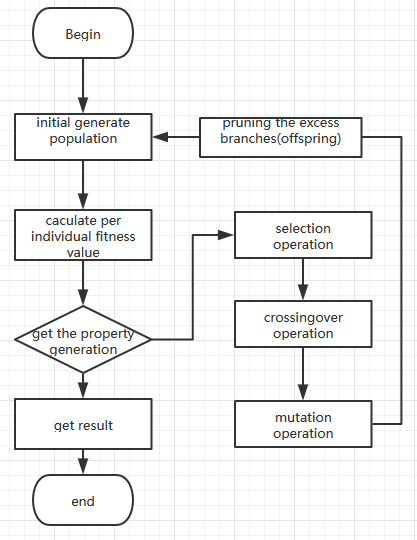
\includegraphics{flowchart1}
	\caption{flowchart}
\end{figure}
	\small
	\bibliographystyle{plain}
	\bibliography{1}

%\cite{1}
%\begin{thebibliography}
%\bibliographystyle{plain}
%\bibliography{1}
%\end{thebibliography}
\end{document}



